% Load LaTeX and package
\documentclass[11pt, xcolor=x11names,compress]{beamer}
\usepackage[utf8]{inputenc}
\usepackage{mathtools}  % for paired delimiters 
\usepackage{mathrsfs}   % for script capitals
\usepackage{amsmath}
\usepackage{amssymb}
\usepackage{amsfonts}

\usepackage[dvipsnames]{xcolor} % for color
\usepackage{ragged2e} % for text alignment
\usepackage{dsfont} % for sepecial font (mathds)

\usepackage[labelformat=empty]{caption}

\usepackage{threeparttable} 
\usepackage{makecell} 
\usepackage{wrapfig}

\usepackage{tikz} % highlight
\newcommand*{\yellowemph}[1]{%
\tikz[baseline]\node[rectangle, fill=yellow, rounded corners, inner sep=0.3mm,anchor=base]{#1};%
}

\usepackage{natbib}
\bibliographystyle{abbrvnat}
% Customize theme attributes
\setbeamertemplate{headline}[default]
%% Hide navigation symbols
\setbeamertemplate{navigation symbols}{}
%%\mode<beamer>{\setbeamertemplate{blocks}[rounded][shadow=true]} %for block
%% Outer theme
\useoutertheme{infolines}
\useoutertheme[subsection=false]{miniframes}

%% Inner theme
\useinnertheme{}

% Define template colors
\usecolortheme{rose}
%\usecolortheme{default}

% These are my colors -- there are many like them, but these ones are mine.
\definecolor{blue}{RGB}{0,114,178}
\definecolor{red}{RGB}{213,94,0}
\definecolor{yellow}{RGB}{240,228,66}
\definecolor{green}{RGB}{0,158,115}

\definecolor{UniColor}{RGB}{0,0, 255}
\setbeamercolor{structure}{bg=white, fg=UniColor}
\setbeamercolor{title}{bg = white, fg = UniColor}
\setbeamercolor{author}{bg = white, fg = UniColor}

\DeclareMathOperator{\Var}{\text{Var}}
\DeclareMathOperator{\E}{\text{E}}
\DeclareMathOperator{\Cov}{\text{Cov}}
\DeclareMathOperator{\Corr}{\text{Corr}}

%------------------------------------------------------------
%This block of code defines the information to appear in the
%Title page


\title [ECON 4003: Empirical Exercise 5]{ECON 4003 Econometrics I}

\vspace{10mm}

\author[]{Empirical Exercise 5}
\date[]{\textit{By Duong Trinh}}

%End of title page configuration block
%---------------------------------------------------- 

\begin{document}
\setbeamertemplate{caption}[numbered]
%The next statement creates the title page.
{\titlegraphic{
\includegraphics[scale = 0.05]{GlaLogo.pdf}}
\frame{\titlepage}}

%---------------------------------------------------------

\begin{frame}[fragile,t]
\linespread{1.3}
\frametitle{Picture the Scenario}
\begin{itemize}
    \item \textbf{Objective:} Investigate the effect of smoking on baby's birth weight.
    \item \textbf{Dataset:} \texttt{birthweight\_smoking.dta} 
    \begin{itemize}
        \item [$\square$] a random sample of 3,000 babies born in Pennsylvania in 1989. 
    \end{itemize}
    \item \textbf{Key variables:}
    \begin{itemize}
        \item [$\square$] \texttt{birthweight}: birth weight of infant (in grams) 
        \item [$\square$] \texttt{smoker}: if the mother smoked during pregnancy or not.
        \item [$\square$] \texttt{alcohol}: if the mother drank alcohol during pregnancy or not.
        \item [$\square$] \texttt{nprevist}: total number of prenatal visits.
        \item [$\square$] other various characteristics of the mother.
    \end{itemize}
\end{itemize}
\end{frame}
%---------------------------------------------------------

%---------------------------------------------------------
\begin{frame}[fragile,t]
\frametitle{Question 1} 

\vspace{15mm}

Estimate the following two regression models:
\begin{itemize}
    \item $birthweight_i=\beta_{0}+\beta_{1} smoker_{i}+u_{i}$ \hspace{2mm} (1)
    \item $birthweight_i=\gamma_{0}+\gamma_{1} smoker_{i}+\gamma_{2} alcohol_{i} + \gamma_{3} nprevist_{i} + e_{i}$ \hspace{2mm} (2)
\end{itemize}
\end{frame}
%---------------------------------------------------------

%---------------------------------------------------------
\begin{frame}[fragile,t]
\frametitle{Question (1a) Interpretation} 
\begin{center}
\begin{threeparttable}
\begin{tabular}{lcc}
\hline 
 & \multicolumn{2}{c}{Dependent Variable: Birth Weight} \\ 
\cline{2-3} 
 & (1) & (2)\\ 
\hline 
 Smoker & \textcolor{red}{-253.23}$^{***}$ & \textcolor{green}{-217.58}$^{***}$ \\ 
  & (26.81) & (26.11) \\ 
  Alcohol &  & \textcolor{green}{-30.49} \\ 
  &  & (72.60) \\ 
  Nprevist &  & \textcolor{green}{34.07}$^{***}$ \\ 
  &  & (2.855) \\ 
  Constant & \textcolor{red}{3,432.06}$^{***}$ & \textcolor{green}{3,051.25}$^{***}$ \\ 
  & (11.89) & (43.71) \\ 
 \hline 
$n$ & 3,000 & 3,000 \\ 
$R^{2}$ & 0.029 & 0.073 \\ 
$\overline{R}^{2}$ & 0.028 & 0.072 \\ 
\hline
\end{tabular} 
\begin{tablenotes}[flushleft]
\footnotesize
Note: Standard errors are in parenthesis.\\
$^{*}$p$<$0.1; $^{**}$p$<$0.05; $^{***}$p$<$0.01 \\
\end{tablenotes}
\end{threeparttable}
\end{center}
\end{frame}
%---------------------------------------------------------

%---------------------------------------------------------
\begin{frame}[fragile,t]
\frametitle{Question (1a) Interpretation} 
\textbf{Model 1:}
\begin{equation*}
    \underset{(se)}{\widehat{birthweight}} = \underset{(11.89)}{3432.06} - \underset{(26.81)}{253.23} \cdot smoker
\end{equation*}
\begin{itemize}
    \item The average birth weight of babies born to non-smokers (smoker = 0) is \textcolor{red}{3,432.06} grams.
    \item Babies born to smokers had birth weights that on average were \textcolor{red}{253.23} grams lower than babies born to non-smokers.
\end{itemize}
\end{frame}
%---------------------------------------------------------

%---------------------------------------------------------
\begin{frame}[fragile,t]
\frametitle{Question (1a) Interpretation (cont.)} 
\textbf{Model 2:} 
\begin{equation*}
    \underset{(se)}{\widehat{birthweight}} = \underset{(43.71)}{3051.25} - \underset{(26.11)}{217.58} \cdot smoker - \underset{(72.60)}{30.49}\cdot alcohol + 
    \underset{(2.855)}{34.07}\cdot nprevist
\end{equation*}
\begin{itemize}
\item The expected birth weight of babies born to women who didn’t smoke during her pregnancy, did not drink alcohol, and didn’t visit prenatal care is \textcolor{green}{3051.25} grams.
\item Babies born to smokers had birth weights that were \textcolor{green}{217.58} grams lower than babies born to non-smokers on average, holding other factors constant.
\item Babies born to women who drank alcohol had birth weights that were \textcolor{green}{30.49} grams lower than babies born to women who drank no alcohol on average, holding other factors constant.
\item An extra prenatal care visit is associated with an increase in birth weight by \textcolor{green}{34.07} grams on average, holding other factors constant.
\end{itemize}
\end{frame}
%---------------------------------------------------------

%---------------------------------------------------------
\begin{frame}[fragile,t]
\frametitle{Question (1b) Omitted Variable Bias} \label{OVBb}
Explain why the exclusion of \texttt{alcohol} and \texttt{nprevist} could lead to omitted variable bias in regression model (1).\\
\hyperlink{OVB}{\beamerbutton{OVB}}
\pause

\vspace{3mm}

Check 2 conditions:
\begin{itemize}
    \item Both \textit{alcohol consumption} and \textit{the number of prenatal doctor visits} may have direct effects on \textit{birth weight}.
    \item \textit{Smoking} may be correlated with both \textit{alcohol consumption} and \textit{the number of prenatal doctor visits}. 
\end{itemize}
\end{frame}
%---------------------------------------------------------

%---------------------------------------------------------
\begin{frame}[fragile,t]
\frametitle{Question (1b) Omitted Variable Bias (cont.)} 
\linespread{1.3}
\begin{itemize}
    \item Both \textit{alcohol consumption} and \textit{the number of prenatal doctor visits} may have direct effects on \textit{birth weight}.\\
    Estimation results of Regression model (2):
    \begin{itemize}
        \item [$\square$] $\hat{\gamma}_2 = -30.49$ \Rightarrow $\gamma_2$ is likely to be negative.
        \item [$\square$] $\hat{\gamma}_3 = 34.07$  \Rightarrow $\gamma_3$ is likely to be positive.
    \end{itemize}
    \item \textit{Smoking} may be correlated with both \textit{alcohol consumption} and \textit{the number of prenatal doctor visits}.\\ 
    Regressing \texttt{smoker} on \texttt{alcohol} and \texttt{nprevist}: 
    \begin{itemize}
        \item [$\square$] \texttt{smoker} is positively correlated with \texttt{alcohol}
         \item [$\square$] \texttt{smoker} is negatively correlated with \texttt{nprevist}    
    \end{itemize}
    The estimated coefficients are also statistically significant.
\end{itemize}
\end{frame}
%---------------------------------------------------------

%---------------------------------------------------------
\begin{frame}[fragile,t]
\frametitle{Question (1c) Interpretation - Omitted Variable Bias} 
Is the estimated coefficient of smoking on birth weight in the
model (2) different from model (1)? Does regression model (1)
seem to suffer from omitted variable bias?\\
\pause
\vspace{3mm}
\begin{itemize}
    \item \textbf{Model 1}: \textcolor{red}{$\hat{\beta}_{1} = -253.23$}
    \item \textbf{Model 2}: \textcolor{green}{$\hat{\gamma}_{1} = -217.58$}\\
    
    \vspace{2mm}
    
    \hspace{12mm} $\Longrightarrow$ \textcolor{red}{$\hat{\beta}_{1}$} $<$
    \textcolor{green}{$\hat{\gamma}_{1}$}
\end{itemize}
The simple regression seems suffer from omitted variable bias (biased downward).
\end{frame}
%---------------------------------------------------------

%---------------------------------------------------------
\begin{frame}[fragile,t]
\frametitle{Question (1d) Prediction}
A mother smoked during her pregnancy, did not drink alcohol, and had 8 prenatal care visits. Use the regression to predict the birth weight of the mother’s child.

\pause
\begin{equation*}
    \underset{(se)}{\widehat{birthweight}} = \underset{(43.71)}{3051.25} - \underset{(26.11)}{217.58} \cdot smoker - \underset{(72.60)}{30.49}\cdot alcohol + 
    \underset{(2.855)}{34.07}\cdot nprevist
\end{equation*}
\begin{equation*}
    \underset{(se)}{\widehat{birthweight}} = \underset{(43.71)}{3051.25} - \underset{(26.11)}{217.58} \times 1 - \underset{(72.60)}{30.49}\times 0 + 
    \underset{(2.855)}{34.07}\times 8 = 3106.23
\end{equation*}

\end{frame}
%---------------------------------------------------------

%---------------------------------------------------------
\begin{frame}[fragile,t]
\frametitle{Question (1e) $R^2$ and adjusted $R^2$}\label{R2b}
Why are the $R^2$ and $\bar{R}^2$ in model (2) so similar?
\hyperlink{R2}{\beamerbutton{R2}}
\begin{center}
\begin{threeparttable}
\begin{tabular}{lcc}
\hline 
 & \multicolumn{2}{c}{Dependent Variable: Birth Weight} \\ 
\cline{2-3} 
 & (1) & (2)\\ 
\hline 
 Smoker & -253.23$^{***}$ & -217.58$^{***}$ \\ 
  & (26.81) & (26.11) \\ 
  Alcohol &  & -30.49\\ 
  &  & (72.60) \\ 
  Nprevist &  & 34.07$^{***}$ \\ 
  &  & (2.855) \\ 
  Constant & 3,432.06$^{***}$ & 3,051.25$^{***}$ \\ 
  & (11.89) & (43.71) \\ 
 \hline 
$n$ & 3,000 & 3,000 \\ 
$R^{2}$ & \textcolor{red}{0.029} & \textcolor{green}{0.073} \\ 
$\overline{R}^{2}$ & \textcolor{red}{0.028} & \textcolor{green}{0.072} \\ 
\hline
\end{tabular} 
\begin{tablenotes}[flushleft]
\end{tablenotes}
\end{threeparttable}
\end{center}

\end{frame}
%---------------------------------------------------------

%---------------------------------------------------------
\begin{frame}[fragile,t]
\frametitle{Question (1e) $R^2$ and adjusted $R^2$}
\linespread{1.3}
Why are the $R^2$ and $\bar{R}^2$ in model (2) so similar?

\vspace{10mm}

\begin{itemize}
    \item They are nearly identical because the sample size is very large ($n = 3000$) and the number of regressors is small ($k = 3$)
\end{itemize}
\end{frame}
%---------------------------------------------------------

%---------------------------------------------------------
\begin{frame}[fragile,t]
\frametitle{Question 2}
\linespread{1.3}
An alternative way to control for prenatal visits is to use the binary variables \texttt{tripre0} through \texttt{tripre3}. Regress \texttt{birthweight} on \texttt{smoker}, \texttt{alcohol}, \texttt{tripre0} , \texttt{tripre2}, and \texttt{tripre3}.

\vspace{3mm}

\begin{itemize}
        \item [$\square$] \texttt{nprevist}: total number of prenatal visits.
        \item [$\square$] \texttt{tripre0}: indicator = 1 if no prenatal visit.
        \item [$\square$] \texttt{tripre1}: indicator = 1 if the first prenatal visit in $1^{st}$ trimester.
        \item [$\square$] \texttt{tripre2}: indicator = 1 if the first prenatal visit in $2^{nd}$ trimester.
        \item [$\square$] \texttt{tripre3}: indicator = 1 if the first prenatal visit in $3^{rd}$ trimester.        
\end{itemize}
\end{frame}
%---------------------------------------------------------

%---------------------------------------------------------
\begin{frame}[fragile,t]
\frametitle{Question (2a) Perfect Multicollinearity} 
Why is \texttt{tripre1} excluded from the regression? What would happen if you included it in the regression?
\pause
\begin{figure}
    \centering
    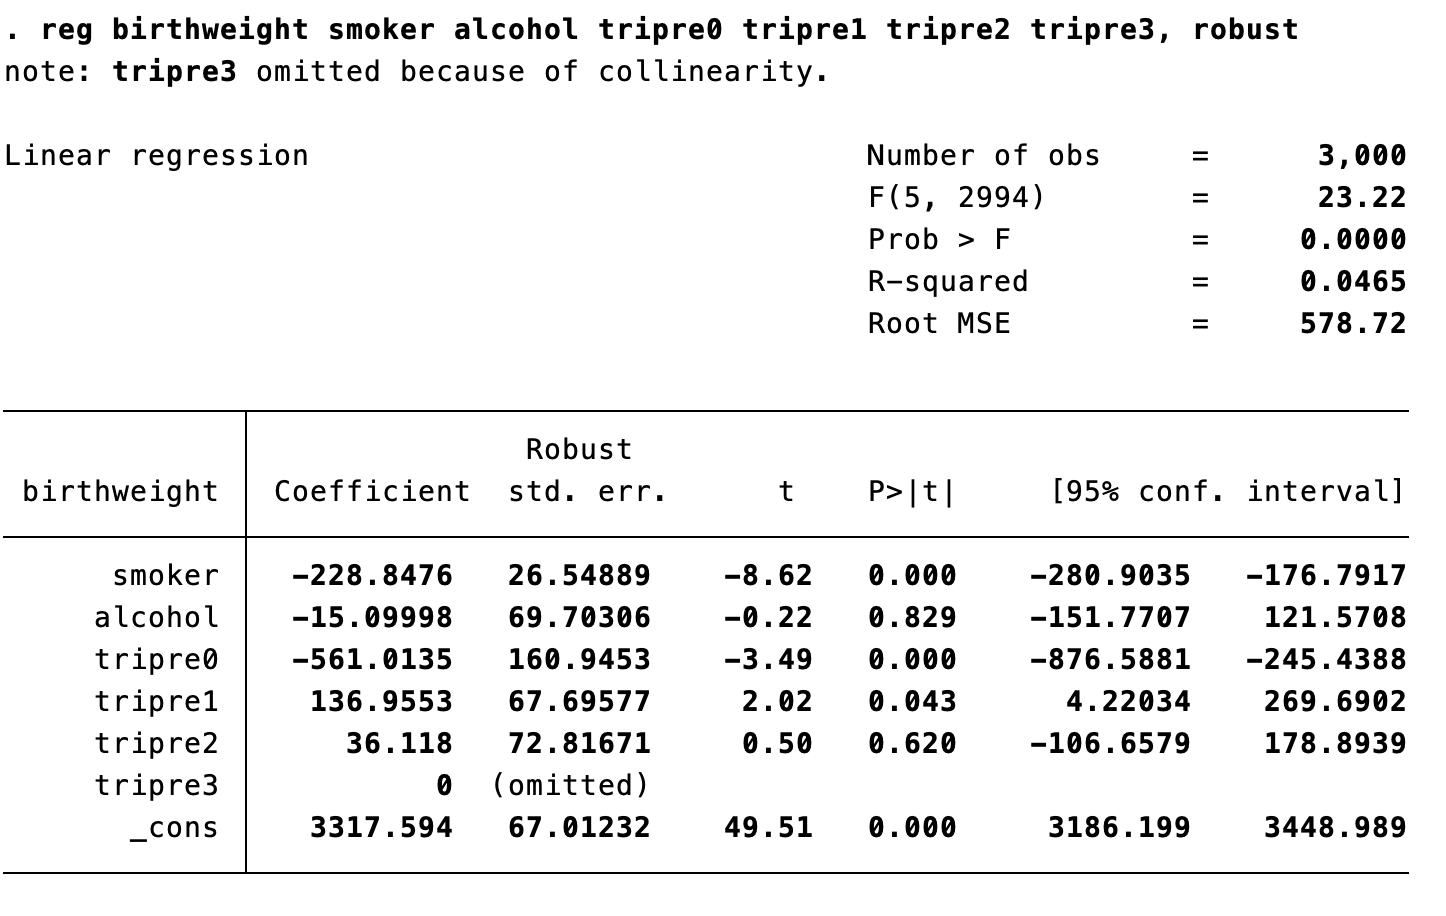
\includegraphics[scale = 0.4]{dummy_trap.png}
    \caption{}
    \label{fig:my_label}
\end{figure}
\end{frame}
%---------------------------------------------------------

%---------------------------------------------------------
\begin{frame}[fragile,t]
\frametitle{Question (2a) Perfect Multicollinearity} 
Why is \texttt{tripre1} excluded from the regression? What would happen if you included it in the regression?

\vspace{5mm}

Let's ask a question...\\

\textbf{When was the first prenatal visit of the woman $i$?
}

\begin{center}
\setlength{\tabcolsep}{3pt}
\begin{tabular}{|c|c|c|c|c|}
\hline
& \texttt{tripre1} & \texttt{tripre2} & \texttt{tripre3} & \texttt{tripre0}
\\
\hline
In $1^{st}$ trimester & \textbf{1} & 0 & 0 & 0
\\
 \hline 
In $2^{nd}$ trimester & 0 & \textbf{1} & 0 & 0
\\
\hline 
In $3^{rd}$ trimester & 0 & 0 & \textbf{1} & 0
\\
\hline 
She had no visit & 0 & 0 & 0 & \textbf{1}
\\ \hline
\end{tabular}
\end{center}

$\Longrightarrow$ Always: $\texttt{tripre0} + \texttt{tripre1} + \texttt{tripre2} + \texttt{tripre3} = 1$
\end{frame}
%---------------------------------------------------------

%---------------------------------------------------------
\begin{frame}[fragile,t]
\frametitle{Question (2a) Perfect Multicollinearity} 
Why is \texttt{tripre1} excluded from the regression? What would happen if you included it in the regression?

\vspace{3mm}
\begin{itemize}
    \item \texttt{tripre1} is omitted to avoid \textcolor{red}{perfect multicollinearity}: This is because \texttt{tripre0} + \texttt{tripre1} + \texttt{tripre2} + \texttt{tripre3} = 1, which equals the value of the ‘constant’ regressor that determines the intercept\\
    $\rightarrow$ one regressor is an exact linear function of the other regressors.\\
    $\rightarrow$ Assumption (MR.3) is violated, the OLS estimator is not defined.
    \item Stata will drop one of the dummy variables if \texttt{tripre0}, \texttt{tripre1}, \texttt{tripre2}, and \texttt{tripre3}, and the constant term all included in the regression.
    
    \item \yellowemph{If there are G dummy variables and each observation falls into one} \yellowemph{and only one category, you will include only G-1 of them as regressors} \yellowemph{to avoid \textbf{dummy variable trap}}
    . 
\end{itemize}
\end{frame}
%---------------------------------------------------------

%---------------------------------------------------------
\begin{frame}[fragile,t]
\frametitle{Question (2b,c) Interpretation} 
$birthweight_i=\eta_{0}+\eta_{1} smoker_{i}+\eta_{2} alcohol_{i} + \alpha_{0} tripre0_{i} + \alpha_{2} tripre2_{i} + \alpha_{3} tripre3_{i}+ e_{i}$

\begin{align*}
    \mathbb{E}[birthweight|\textcolor{red}{tripre1} = 1, smk, alc] &= \eta_{0}+\eta_{1}  smk +\eta_{2} alc\\
    \mathbb{E}[birthweight|\textcolor{green}{tripre0} = 1, smk, alc] &= \eta_{0}+\eta_{1} smk+\eta_{2} alc + \textcolor{green}{\alpha_{0}}\\
    \mathbb{E}[birthweight|\textcolor{green}{tripre2} = 1, smk, alc] &= \eta_{0}+\eta_{1}  smk +\eta_{2} alc + \textcolor{green}{\alpha_{2}}\\
    \mathbb{E}[birthweight|\textcolor{green}{tripre3} = 1, smk, alc] &= \eta_{0}+\eta_{1}  smk+\eta_{2} alc + \textcolor{green}{\alpha_{3}}
\end{align*}
\begin{itemize}
    \item \yellowemph{The coefficients on the \textcolor{green}{\textbf{included dummy variables}} represent the} \yellowemph{\textbf{incremental effect} of being in that category, relative to the base} \yellowemph{case of the \textcolor{red}{\textbf{omitted category}}, holding constant the other regressors.}
\end{itemize}

\end{frame}
%---------------------------------------------------------

%---------------------------------------------------------
\begin{frame}[fragile,t]
\frametitle{Question (2b,c) Interpretation} 
\begin{center}
\begin{threeparttable}
\begin{tabular}{lc} 
\hline 
 & \multicolumn{1}{c}{Dependent Variable: Birth Weight} \\ 
\cline{2-2} 
 & (1) \\ 
\hline 
 Smoker & -228.85 (26.55) $^{***}$ \\ 
  Alcohol & -15.10 (69.70)\\ 
  \textcolor{green}{Tripre0} & \textcolor{green}{-697.97} (146.58)$^{***}$ \\ 
  \textcolor{green}{Tripre2} & \textcolor{green}{-100.84} (31.55)$^{***}$ \\ 
  \textcolor{green}{Tripre3} & \textcolor{green}{-136.96} (67.70)$^{**}$ \\ 
  Constant & 3,454.55 (12.48)$^{***}$ \\ 
 \hline 
$n$ & 3,000\\
$R^{2}$ & 0.046 \\
$\overline{R}^{2}$ & 0.045 \\
\hline 
\end{tabular} 
\begin{tablenotes}[flushleft]
\footnotesize
Note: Standard errors are in parenthesis. \\
$^{*}$p$<$0.1; $^{**}$p$<$0.05; $^{***}$p$<$0.01 \\ 
\end{tablenotes}
\end{threeparttable}
\end{center}
\end{frame}
%---------------------------------------------------------

%---------------------------------------------------------
\begin{frame}[fragile,t]
\frametitle{Question (2b,c) Interpretation} 
\begin{center}
\begin{threeparttable}
\begin{tabular}{lc} 
\hline 
 & \multicolumn{1}{c}{Dependent Variable: Birth Weight} \\ 
\cline{2-2} 
 & (1) \\ 
\hline 
 Smoker & -228.85 (26.55) $^{***}$ \\ 
  Alcohol & -15.10 (69.70)\\ 
  \textcolor{green}{Tripre0} & \textcolor{green}{-697.97} (146.58)$^{***}$ \\ 
  Tripre2 & -100.84 (31.55)$^{***}$ \\ 
  Tripre3 & -136.96 (67.70)$^{**}$ \\ 
  Constant & 3,454.55 (12.48)$^{***}$ \\ 
\hline 
\end{tabular} 
\begin{tablenotes}[flushleft]
\footnotesize
Note: Standard errors are in parenthesis. \\
$^{*}$p$<$0.1; $^{**}$p$<$0.05; $^{***}$p$<$0.01 \\ 
\end{tablenotes}
\end{threeparttable}
\end{center}
Babies born to women who had no prenatal doctor visits (\textcolor{green}{tripre0} = 1) had birth weights that were on average 697.97 grams lower than babies from others
who saw a doctor during the first trimester (\textcolor{red}{tripre1} = 1).
\end{frame}
%---------------------------------------------------------

%---------------------------------------------------------
\begin{frame}[fragile,t]
\frametitle{Question (2b,c) Interpretation} 
\begin{center}
\begin{threeparttable}
\begin{tabular}{lc} 
\hline 
 & \multicolumn{1}{c}{Dependent Variable: Birth Weight} \\ 
\cline{2-2} 
 & (1) \\ 
\hline 
 Smoker & -228.85 (26.55) $^{***}$ \\ 
  Alcohol & -15.10 (69.70)\\ 
  Tripre0 & -697.97 (146.58)$^{***}$ \\ 
  \textcolor{green}{Tripre2} & \textcolor{green}{-100.84} (31.55)$^{***}$ \\ 
  Tripre3 & -136.96 (67.70)$^{**}$ \\ 
  Constant & 3,454.55 (12.48)$^{***}$ \\ 
 \hline 
\end{tabular} 
\begin{tablenotes}[flushleft]
\footnotesize
Note: Standard errors are in parenthesis. \\
$^{*}$p$<$0.1; $^{**}$p$<$0.05; $^{***}$p$<$0.01 \\ 
\end{tablenotes}
\end{threeparttable}
\end{center}
Babies born to women whose first doctor visit was during the
second trimester ( \textcolor{green}{tripre2} = 1) had birth weights that on average
were 100.84 grams lower than babies from others who saw a
doctor during the first trimester ( \textcolor{red}{tripre1} = 1).
\end{frame}
%---------------------------------------------------------

%---------------------------------------------------------
\begin{frame}[fragile,t]
\frametitle{Question (2b,c) Interpretation} 
\begin{center}
\begin{threeparttable}
\begin{tabular}{lc} 
\hline 
 & \multicolumn{1}{c}{Dependent Variable: Birth Weight} \\ 
\cline{2-2} 
 & (1) \\ 
\hline 
 Smoker & -228.85 (26.55) $^{***}$ \\ 
  Alcohol & -15.10 (69.70)\\ 
  Tripre0 & -697.97 (146.58)$^{***}$ \\ 
  Tripre2 & -100.84 (31.55)$^{***}$ \\ 
  \textcolor{green}{Tripre3} & \textcolor{green}{-136.96} (67.70)$^{**}$ \\ 
  Constant & 3,454.55 (12.48)$^{***}$ \\ 
 \hline 
\end{tabular} 
\begin{tablenotes}[flushleft]
\footnotesize
Note: Standard errors are in parenthesis. \\
$^{*}$p$<$0.1; $^{**}$p$<$0.05; $^{***}$p$<$0.01 \\ 
\end{tablenotes}
\end{threeparttable}
\end{center}
Babies born to women whose first doctor visit was during the third
trimester (\textcolor{green}{tripre3} = 1) had birth weights that on average were
136.96 grams lower than babies from others who saw a doctor
during the first trimester (\textcolor{red}{tripre1} = 1).
\end{frame}
%---------------------------------------------------------

%---------------------------------------------------------
\begin{frame}[fragile,t]
\frametitle{Question (2d)} 
\linespread{1.3}
Does the regression model in Q2 explain a larger fraction of the
variance in birth weight than the second regression model in Q1?

\pause

\vspace{3mm}

\begin{itemize}
    \item \textbf{Q2 - Model:}\\
$birthweight_i=\eta_{0}+\eta_{1} smoker_{i}+\eta_{2} alcohol_{i} + \alpha_{0} tripre0_{i} + \alpha_{2} tripre2_{i} + \alpha_{3} tripre3_{i}+ e_{i}$\\
    Estimation results: $R^2 = 0.046$, $\overline{R}^2 = 0.045$
    \item \textbf{Q1 - Model 2:}\\
$birthweight_i=\gamma_{0}+\gamma_{1} smoker_{i}+\gamma_{2} alcohol_{i} + \gamma_{3} nprevist_{i} + e_{i}$
    Estimation results: $R^2 = 0.073$, $\overline{R}^2 = 0.072$
\end{itemize}

\vspace{3mm}

$\Longrightarrow$ Both $R^2$ and $\overline{R}^2$ are lower in Q2.
\end{frame}
%---------------------------------------------------------

%---------------------------------------------------------
\begin{frame}[fragile,t]
\frametitle{Appendix: Omitted Variable Bias}\label{OVB}
For omitted variable bias occur, the omitted variable $Z$ must satisfy \textbf{both} conditions:
\begin{itemize}
    \item $Z$ is a determinant of $Y$; and
    \item $Z$ is correlated with the regressor X
\end{itemize}
\begin{figure}
    \centering
    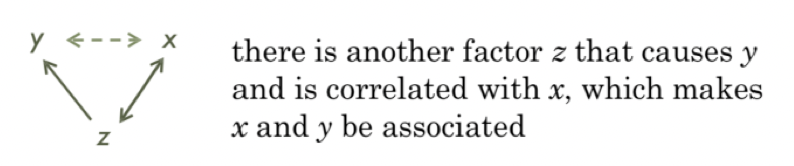
\includegraphics[scale=0.6]{OVB.png}
    \caption{}
    \label{fig:my_label}
\end{figure}
 \end{frame}
%---------------------------------------------------------

%---------------------------------------------------------
\begin{frame}[fragile,t]
\frametitle{Appendix: Omitted Variable Bias (cont.)}\label{OVB}
\begin{equation*}
    plim\hat{\beta_1} = \beta_1 + \beta_2\frac{Cov(X,Z)}{Var(X)}
\end{equation*}

\begin{itemize}
    \item $\hat{\beta_1}$ is biased \textcolor{red}{upward} \hspace{3mm} $\Leftrightarrow$ \textcolor{red}{$plim\hat{\beta_1} > \beta_1$}
    \item $\hat{\beta_1}$ is biased \textcolor{green}{downward} $\Leftrightarrow$ \textcolor{green}{$plim\hat{\beta_1} < \beta_1$}
\end{itemize}

\vspace{3mm}

\begin{center}
\setlength{\tabcolsep}{3pt}
\begin{tabular}{|c|c|c|}
\hline
& $Cov(X,Z) > 0$ & $Cov(X,Z) < 0$
\\
\hline
$\beta_2 > 0$ & \textcolor{red}{$plim\hat{\beta_1} > \beta_1$}  & \textcolor{green}{$plim\hat{\beta_1} < \beta_1$} \\
 \hline 
$\beta_2 < 0$ & \textcolor{green}{$plim\hat{\beta_1} < \beta_1$} & \textcolor{red}{$plim\hat{\beta_1} > \beta_1$}
\\ \hline
\end{tabular}
\end{center}
\hyperlink{OVBb}{\beamerbutton{Back}}
 \end{frame}
%---------------------------------------------------------

%---------------------------------------------------------
\begin{frame}[fragile,t]
\frametitle{Appendix: Omitted Variable Bias (cont.)}\label{OVB}
\begin{equation*}
    plim\hat{\beta_1} = \beta_1 + \beta_2\frac{Cov(X,Z)}{Var(X)} + \beta_3\frac{Cov(X,W)}{Var(X)}
\end{equation*}

\begin{itemize}
    \item $\hat{\beta_1}$ is biased \textcolor{red}{upward} \hspace{3mm} $\Leftrightarrow$ \textcolor{red}{$plim\hat{\beta_1} > \beta_1$}
    \item $\hat{\beta_1}$ is biased \textcolor{green}{downward} $\Leftrightarrow$ \textcolor{green}{$plim\hat{\beta_1} < \beta_1$}
\end{itemize}
 \end{frame}
%---------------------------------------------------------

%---------------------------------------------------------
\begin{frame}[fragile,t]
\frametitle{Appendix: $R^2$ and adjusted $R^2$}\label{R2}
\begin{itemize}
    \item $R^{2}$ is the fraction of the sample variance of $Y$ explained by $X$
$$
R^{2}=\frac{\sum_{i=1}^{n}\left(\widehat{Y}_{i}-\bar{Y}\right)^{2}}{\sum_{i=1}^{n}\left(Y_{i}-\bar{Y}\right)^{2}}=\frac{\text { Explained sum of squares (ESS) }}{\text { Total sum of squares (TSS) }}
$$
    \item Adjusted $R^{2}\left(\right.$ or $\left.\bar{R}^{2}\right)$ takes $R^{2}$ and penalise for additional regressors
$$
\bar{R}^{2}=1-\left(\frac{n-1}{n-k-1}\right) \frac{S S R}{T S S}=1-\left(\frac{n-1}{n-k-1}\right)\left(1-R^{2}\right)
$$
    \begin{itemize}
        \item [$\square$] $\frac{n-1}{n-k-1}$ is greater than 1 and grows with $k$
        \item [$\square$] $\bar{R}^{2}<R^{2}$, however two will be very close if $n$ is large, $k$ is small, or $R^{2}=0$ (which is very unlikely)
    \end{itemize}
\end{itemize}
\hyperlink{R2b}{\beamerbutton{Back}}
 \end{frame}
%---------------------------------------------------------

%---------------------------------------------------------
\end{document}